\phantomsection
\section*{Analisi del Rischio}
\addcontentsline{toc}{section}{Analisi del Rischio}

\phantomsection
\addcontentsline{toc}{subsection}{Valutazione dei beni}

\rowcolors{2}{white!0!}{orange!10!}

\begin{adjustwidth}{-1.5cm}{0cm}

\resizebox{1.3\textwidth}{!}{
\begin{tabular}{ |l|l|l|  }
\hline
\rowcolor{red!80!}\multicolumn{3}{|c|}{\huge\textbf{\textcolor{white}{Valutazione dei beni}}} \\
\hline
\rowcolor{red!70!}\Large\textbf{\textcolor{white}{Bene}} & \Large\textbf{\textcolor{white}{Valore}} & \Large\textbf{\textcolor{white}{Esposizione}}\\
\hline

\textbf{Sistema Informativo} &
\begin{tabular}{@{}l@{}}
Alto.\\ Supporto alla gestione\\
dei dati utilizzati in molte delle funzionalità offerte\\ dal sistema.
\end{tabular} &
\begin{tabular}{@{}l@{}}
Alta.\\
Perdita economica e costi di ripristino.\\ 
Perdita d’immagine se la notizia diventa di\\
pubblico dominio.
\end{tabular} \\

\textbf{\begin{tabular}{@{}l@{}}
Informazioni relative \\agli utenti.
\end{tabular}}  &
\begin{tabular}{@{}l@{}}
Medio-Alto.\\
Informazioni relative agli utenti del sistema,\\
anche le credenziali,le quali\\ potrebbero permettere l’accesso ai file personali e di gruppo
\end{tabular} &
\begin{tabular}{@{}l@{}}
Medio-Alta.\\
Perdita d'immagine del Software, possibile\\
perdita dei file personali e di gruppo
\end{tabular} \\

\textbf{\begin{tabular}{@{}l@{}}
Informazioni relative \\all' amministratore
\end{tabular}} &
\begin{tabular}{@{}l@{}}
Molto Alto.\\ Ha completa gestione sugli utenti e sui gruppi
\end{tabular} &
\begin{tabular}{@{}l@{}}
Molto Alta.\\
Possibilità di compromettere l'intero sistema,\\
perdita dei dati e dei file.\\
Perdita d'immmagine del Software 
\end{tabular} \\


\textbf{Informazioni contenute nei file} &
\begin{tabular}{@{}l@{}}
Alto.\\ Informazioni private di utenti e gruppi.
\end{tabular} &
\begin{tabular}{@{}l@{}}
Alto.\\
Perdita d'immagine del Software, possibile \\perdita dei file personali e di gruppo 
\end{tabular} \\

\hline
\end{tabular}
}

\end{adjustwidth}




\pagebreak
\phantomsection
\addcontentsline{toc}{subsection}{Analisi minacce e controlli}

\rowcolors{2}{white!0!}{orange!10!}

\begin{adjustwidth}{-2cm}{0cm}

\resizebox{1.3\textwidth}{!}{
\begin{tabular}{ |l|l|l|l|  }
\hline
\rowcolor{red!80!}\multicolumn{4}{|c|}{\huge\textbf{\textcolor{white}{Analisi minacce e controlli}}} \\
\hline
\rowcolor{red!70!}\Large\textbf{\textcolor{white}{Minaccia}} & \Large\textbf{\textcolor{white}{Probabilità}} & \Large\textbf{\textcolor{white}{Controllo}} &
\Large\textbf{\textcolor{white}{Fattibilità}} \\
\hline

\begin{tabular}{@{}l@{}}
Furto d'identità \\(utente).
\end{tabular} & 
\begin{tabular}{@{}l@{}}
Media.\\ Username e password scelti \\
dall'utente potrebbero essere utilizzati\\
in altre applicazioni vulnerabili.
\end{tabular} &
\begin{tabular}{@{}l@{}}
Dopo alcuni tentativi errati viene \\
bloccato l’accesso.\\
Log di ogni operazione e degli indirizzi IP.
\end{tabular} & 
\begin{tabular}{@{}l@{}}
Basso costo di implementazione.
\end{tabular} \\

\begin{tabular}{@{}l@{}}
Furto d'identità \\(aministratore).
\end{tabular} & 
\begin{tabular}{@{}l@{}}
Bassa.\\
Username e password stabiliti\\
dall'amministratore,\\ numero di accessi limitato.\\
\end{tabular} &
\begin{tabular}{@{}l@{}}
Dopo alcuni tentativi errati viene \\
bloccato l’accesso.\\
Log di ogni operazione e degli indirizzi IP.
\end{tabular} & 
\begin{tabular}{@{}l@{}}
Basso costo di implementazione, \\
prestare attenzione all'accesso\\
ai dispositivi autenticati.
\end{tabular} \\

\begin{tabular}{@{}l@{}}
Intercettazione delle comunicazioni.
\end{tabular} &
\begin{tabular}{@{}l@{}}
Media.\\
Il servizio è realizzato in rete interna.
\end{tabular} &
\begin{tabular}{@{}l@{}}
Utilizzo di un sistema crittografico per la\\
cifratura delle comunicazioni.
\end{tabular} &
\begin{tabular}{@{}l@{}}
Basso costo, utilizzo di crittografia\\
simmetrica o asimmetrica.
\end{tabular}\\

\begin{tabular}{@{}l@{}}
Deny of Service
\end{tabular} &
\begin{tabular}{@{}l@{}}
Bassa.\\
poca probabilità di un attacco\\
DoS interno.
\end{tabular} &
\begin{tabular}{@{}l@{}}
- Progettazione adeguata e numero di\\
  operazioni di rete limitato.\\
- Log delle richieste.
\end{tabular} &
\begin{tabular}{@{}l@{}}
Basso costo, gestione delle richieste\\
e della rete delegata all' amministratore.
\end{tabular} 
\\

\begin{tabular}{@{}l@{}}
Furto o modifica dei file
\end{tabular} &
\begin{tabular}{@{}l@{}}
Bassa.\\
difficile accedere \\
al file system dall'esterno.
\end{tabular} &
\begin{tabular}{@{}l@{}}
- Cifratura dei file\\
- Backup periodico
\end{tabular} &
\begin{tabular}{@{}l@{}}
Medio-Alto.\\
Cifratura dei file\\
potrebbe essere onerosa per il sistema.\\
Il backup periodico richiede\\
ulteriore spazio di archiviazione.
\end{tabular} 
\\

\hline
\end{tabular}
}

\end{adjustwidth}



\phantomsection
\addcontentsline{toc}{subsection}{Analisi tecnologica della sicurezza}

\rowcolors{2}{white!0!}{orange!10!}

\begin{adjustwidth}{-1cm}{0cm}

\resizebox{1.1\textwidth}{!}{
\begin{tabular}{ |l|l|  }
\hline
\rowcolor{red!80!}\multicolumn{2}{|c|}{\huge\textbf{\textcolor{white}{Analisi tecnologica della sicurezza}}} \\
\hline
\rowcolor{red!70!}\Large\textbf{\textcolor{white}{Tecnologia}} & \Large\textbf{\textcolor{white}{Vulnerabilità}} \\
\hline


\begin{tabular}{@{}l@{}}
Autenticazione \\
Username/Password
\end{tabular} &
\begin{tabular}{@{}l@{}}
- Password banali\\
- Utente rivela username e password\\
  volontariamente o con attacchi di\\
  ingegneria sociale.\\
- Attacco bruteforce sulle credenziali.
\end{tabular} 
\\

\begin{tabular}{@{}l@{}}
Cifratura della comunicazione\\
dei dati e dei file
\end{tabular} &
\begin{tabular}{@{}l@{}}
Cifratura Simmetrica:\\
\quad - Tempo di vita della chiave. Più \\
\quad informazioni cifro con la stessa chiave \\
\quad più materiale offro per l’analisi del \\
\quad testo ad un attaccante \\
\quad - Lunghezza chiave\\
\quad - Memorizzazione chiave\\
\\
Cifratura Asimmetrica:\\
\quad - Memorizzazione chiave\\
\end{tabular} 
\\

\begin{tabular}{@{}l@{}}
Architettura Client/Server \\
\end{tabular} &
\begin{tabular}{@{}l@{}}
- Vari tipi di attacchi Deny of Service.\\
- Intercettazione delle comunicazioni: \\
attacco Man in The Middle, Sniffing.

\end{tabular} 
\\




\hline
\end{tabular}
}

\end{adjustwidth}



\phantomsection
\section*{Security Use Case e Misuse Case}
\addcontentsline{toc}{subsection}{Security Use Case e Misuse Case}
\begin{adjustwidth}{-2cm}{0cm}
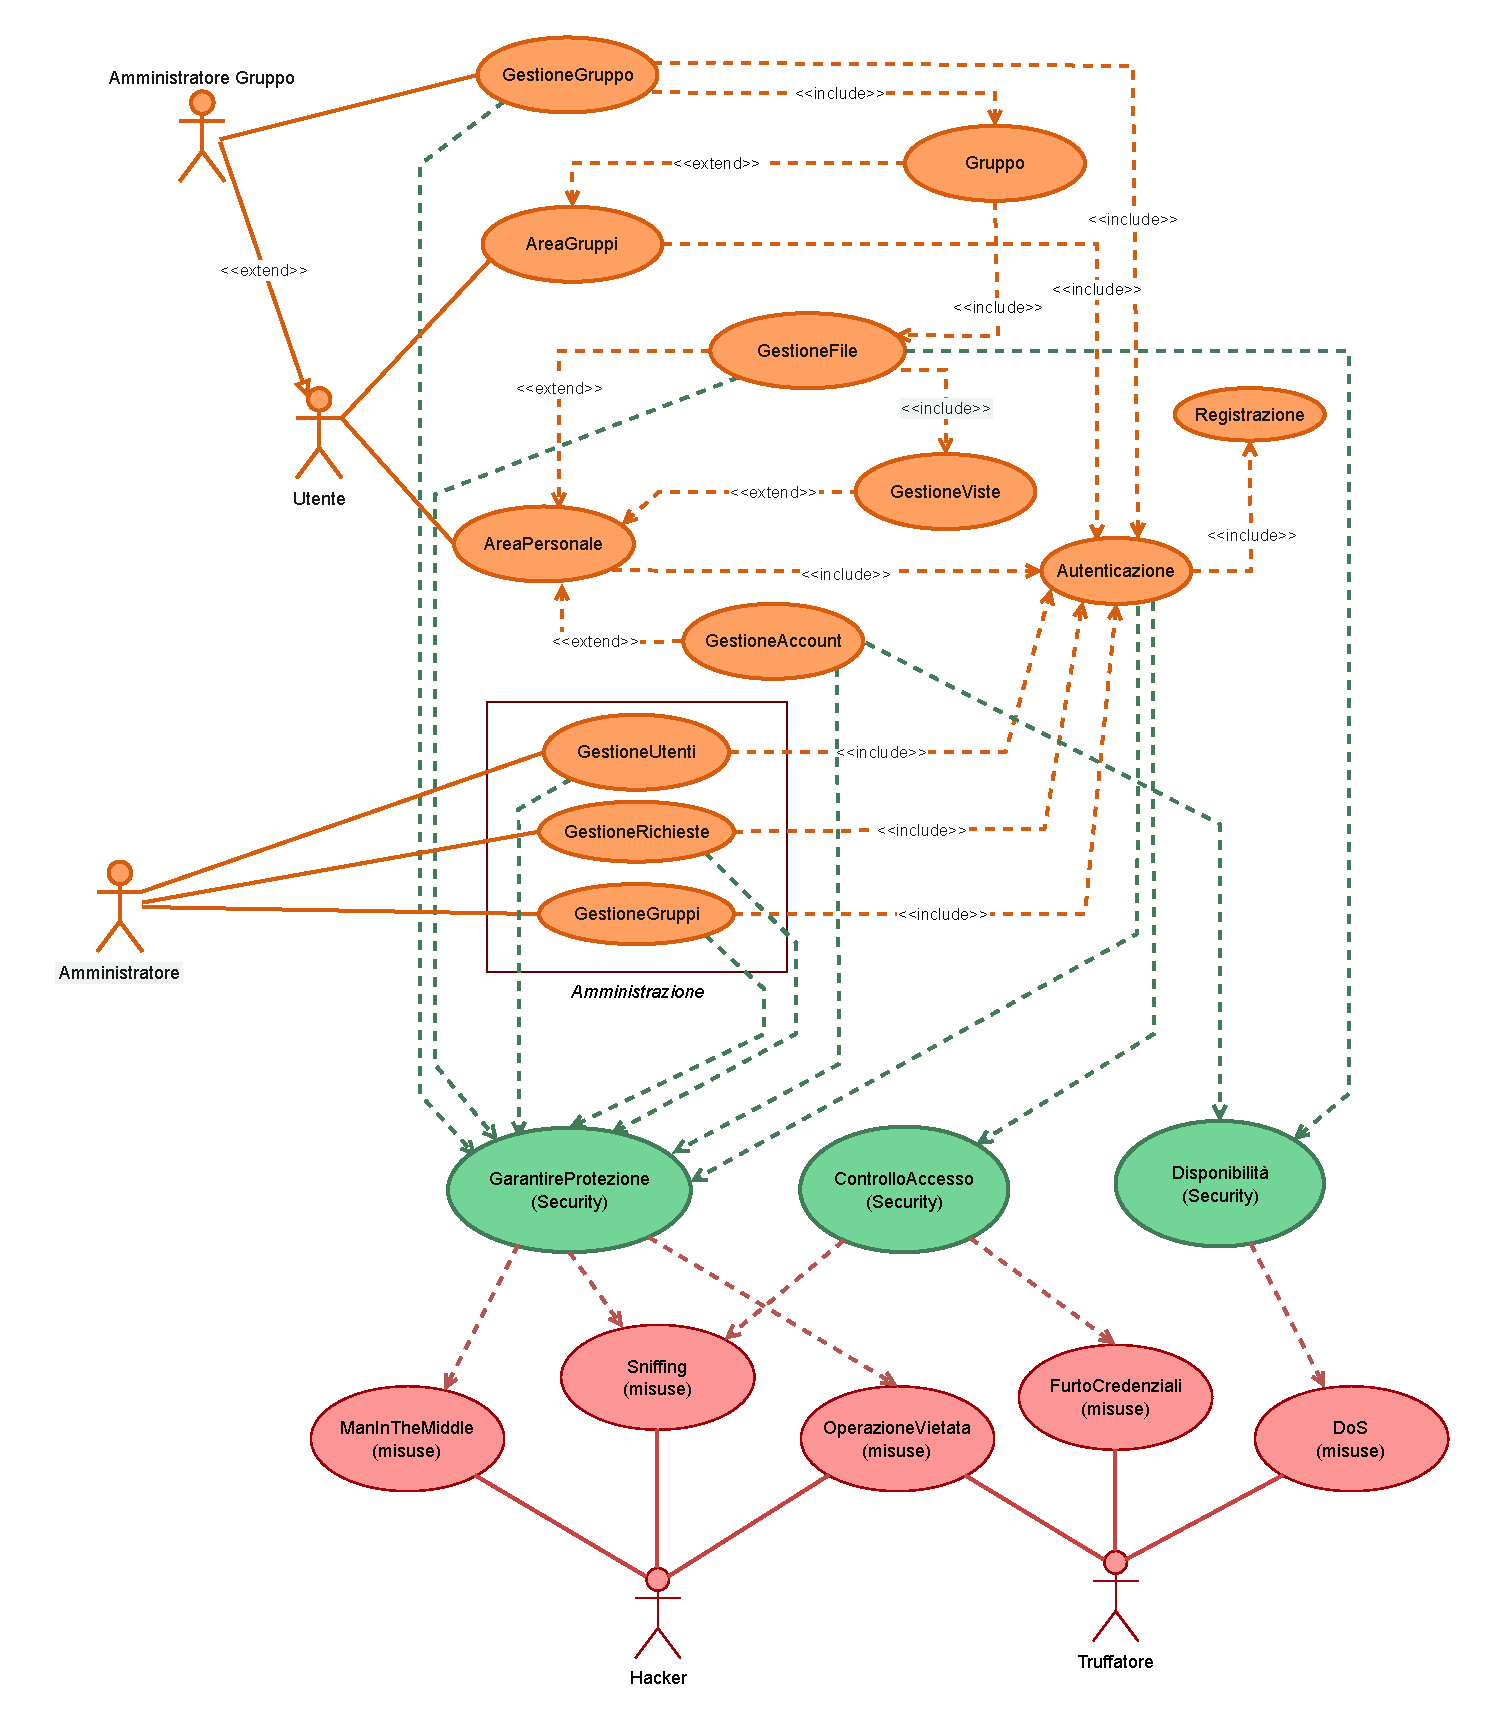
\includegraphics[scale=0.7]{casi d'uso/Casi d'uso-Casi d'uso e misuso.drawio.pdf}
\end{adjustwidth}




\phantomsection
\subsection*{Security Use Case e Misuse Case scenari}
\addcontentsline{toc}{subsection}{Security Use Case e Misuse Case scenari}

\rowcolors{2}{white!0!}{white!0!}


%------------------------------------

\phantomsection
\addcontentsline{toc}{subsubsection}{GarantireProtezione}

\begin{adjustwidth}{-1.5cm}{0cm}
\resizebox{1.2\textwidth}{!}{
\begin{tabular}{ |l|p{5cm}|p{5cm}|  }
\hline
\rowcolor{orange!45}\large\textbf{Titolo} & \multicolumn{2}{c|}{
 \large\textbf{GarantireProtezione}}\\
\hline

\textbf{Descrizione} & \multicolumn{2}{l|}{
Le comunicazioni e i file devono essere protetti }\\
\hline
\textbf{Misuse case} & \multicolumn{2}{l|}{
 ManInTheMiddle, Sniffing, OperazioneVietata }\\
\hline
\textbf{Precondizioni} &
\multicolumn{2}{p{10cm}|}{
L'attaccante o il truffatore ha i mezzi per attuare uno sniffing
delle comunicazioni, manomettere le operazioni tra il client e il server
o intaccare la cifratura dei file.
}\\
\hline
\textbf{Postcondizioni} & \multicolumn{2}{l|}{
 Il sistema registra un tentativo di manomissione nei log}\\
\hline
& Sistema & Attaccante\\
\cline{2-3}
&
Cerca di garantire che i dati 
inviati all’Utente siano protetti, cifrati e
non possano essere modificati
& \\
\cline{2-3}
\multirow{-3 }{*}{\textbf{Scenario Principale}} & &
- Cerca di intercettare e manomettere le comunicazioni

- Cerca di estrarre dati o penetrare nel sistema in modo non autorizzato
\\

\hline
& Sistema & Attaccante\\
\cline{2-3}
&
- Garantisce che i dati sensibili ed i file salvati siano cifrati in maniera robusta

- Cerca di garantire la sicurezza da vulnerabilità
& 

\\
\cline{2-3}
\multirow{-3 }{*}{\textbf{Scenari di attacco avvenuto con successo}}
& 
&
- Cerca di bypassare la cifratura per ottenere le inforamzioni sensibili o i file

- Cerca e trova delle vulnerabilità per superare le difese del sistema
\\
\hline

\end{tabular}}
\end{adjustwidth}
\pagebreak


%------------------------------------

\phantomsection
\addcontentsline{toc}{subsubsection}{ControlloAccesso}

\begin{adjustwidth}{-1.5cm}{0cm}
\resizebox{1.2\textwidth}{!}{
\begin{tabular}{ |l|p{5cm}|p{5cm}|  }
\hline
\rowcolor{orange!45}\large\textbf{Titolo} & \multicolumn{2}{c|}{
 \large\textbf{ControlloAccesso}}\\
\hline

\textbf{Descrizione} & \multicolumn{2}{l|}{
L'accesso al servizio deve essere granulare e monitorato
 }\\
\hline
\textbf{Misuse case} & \multicolumn{2}{l|}{
 FurtoCredenziali, Sniffing }\\
\hline
\textbf{Precondizioni} &
\multicolumn{2}{p{10cm}|}{
L'attaccante dispone di un sistema per attuare un attacco a dizionario
}\\
\hline
\textbf{Postcondizioni} & \multicolumn{2}{l|}{
 Il sistema registra i tentativi ed avverte l'amministratore
 }\\
\hline


& Sistema & Attaccante\\
\cline{2-3}
&
&
Cerca di individuare ed inserire
più volte le Credenziali di un
altro Utente/Amministratore
\\
\cline{2-3}
& 
L'accesso viene negato perché le Credenziali sono errate. Il tentativo di accesso viene registrato in un file di log.
&
\\
\cline{2-3}
\multirow{-4}{*}{\textbf{Scenario Principale}}
& 
Dopo 5 tentativi di accesso errati consecutivi viene bloccato l'accesso
&
\\
\hline



& Sistema & Attaccante\\
\cline{2-3}
&
& 
Accede al sistema
\\
\cline{2-3}
&
Concede l'accesso all'account e ai gruppi a cui l'account è collegato
&
\\
\cline{2-3}
&
&
Cerca di scaricare tutte le informazioni e di enumerare gli utenti
\\
\cline{2-3}
\multirow{-7}{*}{\textbf{Scenari di attacco avvenuto con successo}} 
&
Registra l'accesso nei log
& 
\\
\hline

\end{tabular}}
\end{adjustwidth}
\vspace{0.2cm}




%------------------------------------

\phantomsection
\addcontentsline{toc}{subsubsection}{Disponibilità}

\begin{adjustwidth}{-1.5cm}{0cm}
\resizebox{1.2\textwidth}{!}{
\begin{tabular}{ |l|p{5cm}|p{5cm}|  }
\hline
\rowcolor{orange!45}\large\textbf{Titolo} & \multicolumn{2}{c|}{
 \large\textbf{Disponibilità}}\\
\hline

\textbf{Descrizione} & \multicolumn{2}{l|}{
Il sistema deve sempre fornire servizio
 }\\
\hline
\textbf{Misuse case} & \multicolumn{2}{l|}{
 DoS}\\
\hline
\textbf{Precondizioni} & 
\multicolumn{2}{p{10cm}|}{
L'attaccante dispone di un ambiente per effettuare un attacco efficace
}\\
\hline
\textbf{Postcondizioni} & \multicolumn{2}{p{10cm}|}{
Il sistema monitora il flusso di dati ed eventualmente attua politiche di protezione o ripristino
 }\\
 
\hline

& Sistema & Attaccante\\
\cline{2-3}
&
&
Avvia l'attacco 
\\
\cline{2-3}
\multirow{-2}{*}{\textbf{Scenario Principale}}
&
Registra l'attacco nei log ed eventualmente esegue un ripristino
&
\\
\hline



& Sistema & Attaccante\\
\cline{2-3}
&
&
Riesce a creare un grande flusso di dati
\\
\cline{2-3}
&
Non riesce a contenere l'attacco 
&
\\
\cline{2-3}
&
Non è possibile il ripristino immediato del sistema
&
\\
\cline{2-3}
\multirow{-7}{*}{\textbf{Scenari di attacco avvenuto con successo}} 
&
& 
Riesce a creare un disservizio
\\
\hline



\end{tabular}}
\end{adjustwidth}
\pagebreak




%--------------------------------------------------------

\phantomsection
\addcontentsline{toc}{subsection}{Requisiti Funzionali aggiornati}

\rowcolors{2}{green!0!}{orange!10!}

\begin{adjustwidth}{1cm}{0cm}

\resizebox{0.9\textwidth}{!}{
\begin{tabular}{ |c|p{11cm}|  }
\hline
\rowcolor{blue!55}\multicolumn{2}{|c|}{\Large\textbf{Requisiti Funzionali aggiornati}} \\
\hline
\rowcolor{blue!45}\LARGE{ID} & \LARGE{Requisito}\\
\hline

\textbf{R12F} & Produzione di file di log per tenere traccia delle operazioni.\\
\textbf{R13F} & L'Amministratore può accedere al file di log per controllare e gestire eventuali segnalazione da parte del sistema\\
\textbf{R14F} & Il sistema è protetto da una ACL\\
\textbf{R15F} & Il sistema deve essere in grado di ripristinarsi in seguito ad un attacco DoS\\

\hline
\end{tabular}
}

\end{adjustwidth}
\vspace{1cm}




\phantomsection
\addcontentsline{toc}{subsection}{Requisiti Non Funzionali aggiornati}

\rowcolors{2}{green!0!}{orange!10!}

\begin{adjustwidth}{1cm}{0cm}

\resizebox{0.9\textwidth}{!}{
\begin{tabular}{ |c|p{11cm}|  }
\hline
\rowcolor{purple!55}\multicolumn{2}{|c|}{\Large\textbf{Requisiti Non Funzionali aggiornati}} \\
\hline
\rowcolor{purple!45}\LARGE{ID} & \LARGE{Requisito}\\
\hline

\textbf{R7NF} & Il sistema deve essere in grado di effettuare un ripristino veloce in caso di attacco.\\

\textbf{R8NF} & Backup periodico dei dati.\\
\hline
\end{tabular}
}

\end{adjustwidth}
\vspace{1cm}

%-----------------------------------------------
\phantomsection
\addcontentsline{toc}{subsection}{Vocabolario aggiornato}

\rowcolors{2}{green!0!}{orange!10!}

\begin{adjustwidth}{1cm}{0cm}

\resizebox{0.9\textwidth}{!}{
\Large
\begin{tabular}{ |c|p{8cm}|c|  }
\hline
\rowcolor{red!60}\multicolumn{3}{|c|}{\Large\textbf{Vocabolario aggiornato}} \\
\hline
\rowcolor{red!50}\LARGE{Voce} & \LARGE{Definizione} & \LARGE{Sinonimo}\\
\hline

\textbf{Log} & File in cui vengono registrate le informazioni di Sistema e di Sicurezza & File di log \\

\textbf{ACL} & Sistema che monitora gli accessi & \\
 
\hline
\end{tabular}
}

\end{adjustwidth}
\vspace{1cm}

%-------------------------------------------

\phantomsection
\section*{Casi d'uso aggiornati}
\addcontentsline{toc}{subsection}{Casi d'uso aggiornati}
\begin{adjustwidth}{-2cm}{0cm}
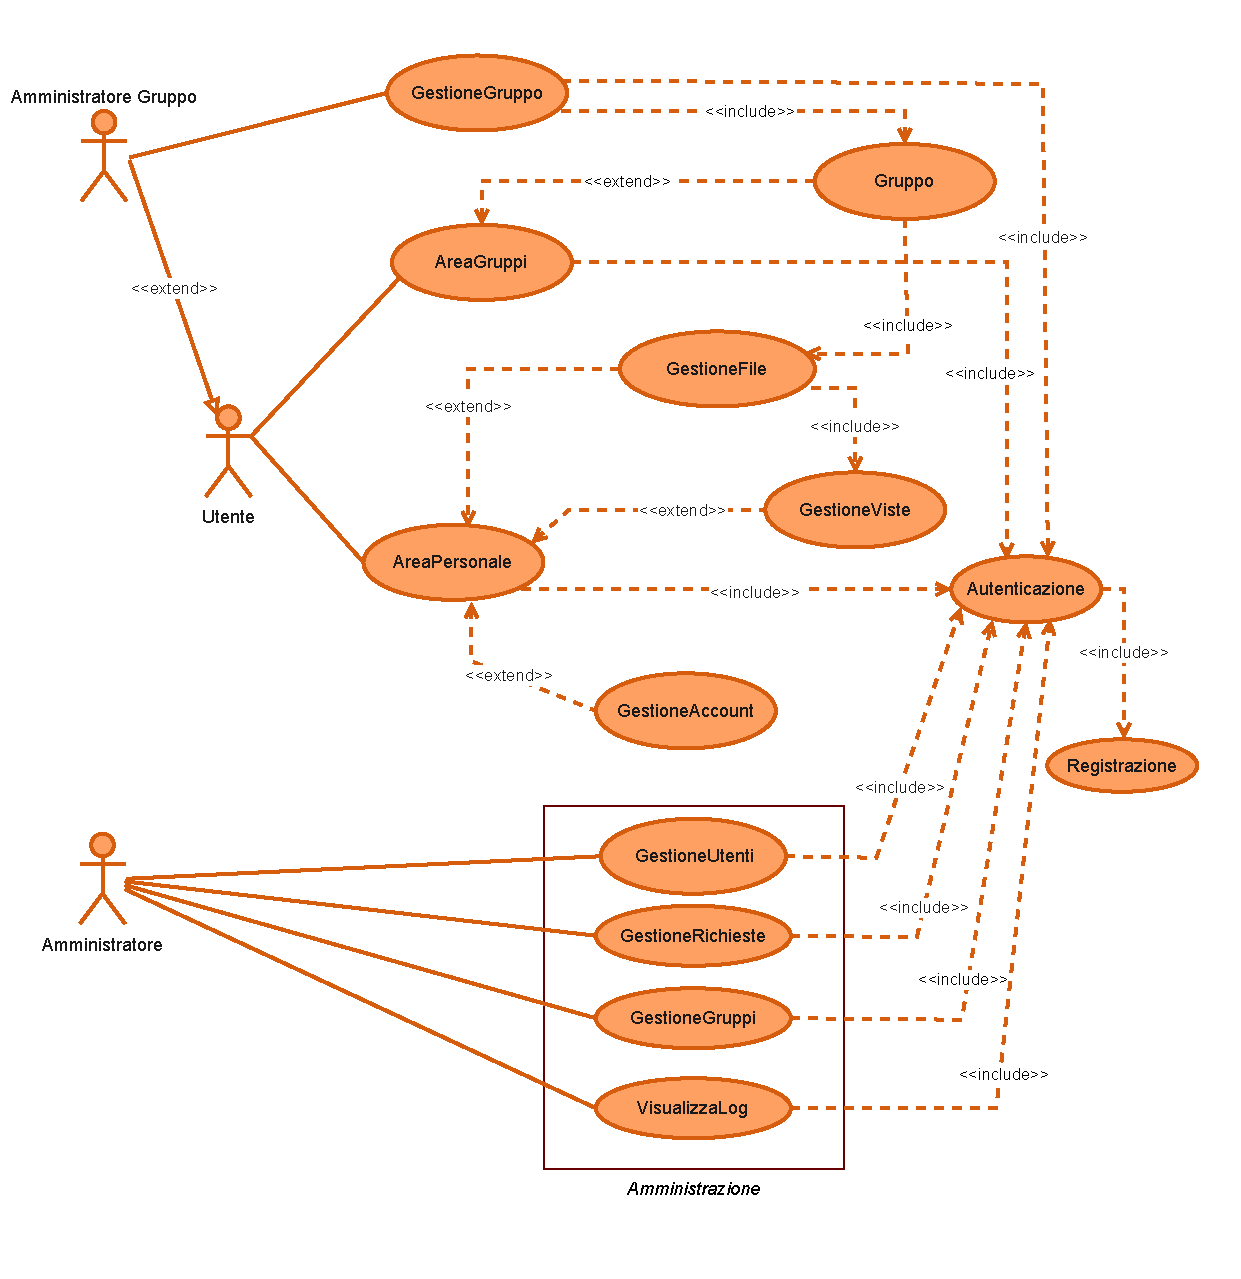
\includegraphics[scale=0.9]{casi d'uso/Casi d'uso-Casi d'uso aggiornati.drawio.pdf}
\end{adjustwidth}



\phantomsection
\addcontentsline{toc}{subsection}{GestioneGruppo}
\rowcolors{2}{white!0!}{white!0!}
\begin{adjustwidth}{0cm}{0cm}

\resizebox{1\textwidth}{!}{
\begin{tabular}{ |l|l|  }
\hline
\rowcolor{red!25}\large\textbf{Titolo} & \large{VisualizzaLog}\\
\hline

\textbf{Descrizione} & Pagina di monitoraggio dei Log\\
\hline
\textbf{Attori} & Amministratore Gruppo\\
\hline
\textbf{Relazioni} & Autenticazione\\
\hline
\textbf{Precondizioni} & \\
\hline
\textbf{Postcondizioni} & \\
\hline
\textbf{Scenario principale} &
\begin{tabular}{@{}l@{}}
1) L'amministratore si autentica\\
2) L'amministratore accede alla sezione dei Log\\
2) L'amministratore del gruppo può visualizzare\\
\quad i Log di sistema
\end{tabular}\\
\hline
\textbf{Scenari alternativi} & \\
\hline
\textbf{Requisiti non funzionali} & \\
\hline
\textbf{Punti aperti} & \\
\hline

\end{tabular}
}
\end{adjustwidth}
\vspace{0.2cm}